\scanpage{57}
\mspage{56}

\uline{Proposition} a) If $F$ \deleted{\unsure{is|was}} is a figure, then the figures $F'$ such that $F'\leq F$ are identified, by the map $F'\mapsto\overline F'$, with the subsets of $\overline F$ which are \uline{closed} for the order relation \inserted{$\leq$} of $M$.

b) If $F$ and $G$ are two figures, $F\wedge G$ exists (infimum for $\leq$) \inserted{\uuline{intersection figure}} and \deleted{\unsure{one|in}} $\overline{F\cap G}=\overline F\cap\overline G$. Same for an arbitrary family $(F_i)_{i\in I}$ \inserted{with 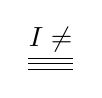
\begin{tikzpicture}[baseline=(f.base)]\node[inner sep=0] (f) {$I\neq\varnothing$};\draw ([yshift=-2pt]f.south west)--([yshift=-2pt]f.south east);\draw ([yshift=-4pt]f.south west)--([yshift=-4pt]f.south east);\draw ([yshift=-6pt]f.south west)--([yshift=-6pt]f.south east);\end{tikzpicture}}.

% Two marginal callout strokes, reproduced beside the associated additions.
\figure{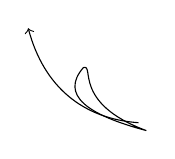
\begin{tikzpicture}[x=1cm,y=1cm]
\draw[->] (1.4,0) .. controls (.7,.05) and (.2,.45) .. (0,1.2);
\draw (1.5,-.1) .. controls (.55,.25) and (.85,.75) .. (.7,.7) .. controls (.4,.35) and (.75,.1) .. (1.5,-.1);
\end{tikzpicture}}
% margin note written sideways
\margin{\uline{But beware} it is better not to denote them by $F\cap G$, for when there is a notion of support, that does not correspond to the intersection of the supports, unless $F,G$ compatible.}

[ \uline{Loci} of $\mathcal F$ : these are the \deleted{\unsure{not|pet}} figures which are \uline{minimal} in $\mathcal F\setminus\{\varnothing_{\mathcal F}\}$. \deleted{A,} \deleted{A loci is of \unsure{this name|name}}  Every locus is irreducible. Thus the loci are also the minimal elements of $ M$ : these are the multistrata which have no strata other than themselves. ] \deleted{If $F$ is a figure, the}

% slanted
\margin{Current definition is reasonable only in certain cases \deleted{(when the} (for example the countries in balls'', or piecewise countries $\ldots$) For in the typical cases of arbitrary order, a \unsure{model|modélé} $\overline E$ \unsure{of str.|of structure} \unsure{semi-}\illegible{1} \inserted{\unsure{empty universes|empty universe},} forms \deleted{\unsure{can be a|can be a}} \inserted{a} \unsure{minimal|very small} multistratum, but one \unsure{calls it|calls} a ``locus'' only if it is \unsure{real void|real void} !}

\uline{Disjoint} \uline{figures} \unsure{,,|''} \uline{$F$} and \uline{$G$} : such that a) $F$ and $G$ compatible, i.e $F\cup G$ exists \deleted{and b)} or again $\{F,G\}$ bounded above for $\leq$ and b) $F\cap G=\varnothing_{\mathcal F}$ \deleted{\unsure{or|and} This means \unsure{thus|that}} \inserted{(i.e. $\overline F\cap\overline G=\varnothing$)}.

% Long curved separator beside the lower margin and proposition.
\figure{\begin{tikzpicture}[x=1cm,y=1cm]\draw (.6,3) .. controls (.2,2.3) and (.05,1.3) .. (.15,.9) .. controls (.2,.3) and (.4,.05) .. (.65,0);\end{tikzpicture}}
% slanted
\margin{blocks my ``\unsure{coproducts|components}''}

\deleted{If $F$ and $G$ are} \uline{Proposition} If $F$ and $G$ are disjoint, then for $F'\leq F$, $G'\leq G$, $F'_{a}$ and $G'$ are disjoint, and $F'\cup G'$ is a subfigure of $F\cup G$, the map $(F';G')\mapsto F'\cup G'$ is a bijection \deleted{from the set of $\unsure{\mathcal F|F}$}
